\documentclass[/home/greg/Thesis/main/main.tex]{subfiles}

%\title{Neutron star mechanics in the observers inertial frame}
%\author{}

\begin{document}
\inputpath{/home/greg/Neutron_star_modelling/AnalysisLyneObservations/}

\newcommand{\Phiexact}{\Phi_{\mathrm{exact}}}
\newcommand{\Phifit}{\Phi_{\mathrm{fit}}}
\newcommand{\wobbleangle}{\tilde{\theta}}
\FloatBarrier

\section{Extracted data}
\graphicspath{{/home/greg/Neutron_star_modelling/ExtractDataFromLyne/img/}}

In this work I am working to test the hypothesis of \citet{Lyne2010} that they
have found compelling evidence for state-switching in at least two pulsars. They
contend that the spin-down rate switched discreetly between two distinct states.
This is not observed in the corresponding measure of $\dot{\nu}$ (see figure 5
from their paper) because of an averaging process. Instead, they consider a
measure of the beam-width $W_{10}$ because this can be measured without averaging.

I have extracted the data for the B1828-11 pulsar from the \citet{Lyne2010}
paper and plotted the $W_{10}$ value in figure \ref{fig: B1828 data}. In future
I intend to apply the same analysis to the other available data sets (3 in total)
but begin with just one to develop the methodology.
\begin{figure}[htb]
    \centering
    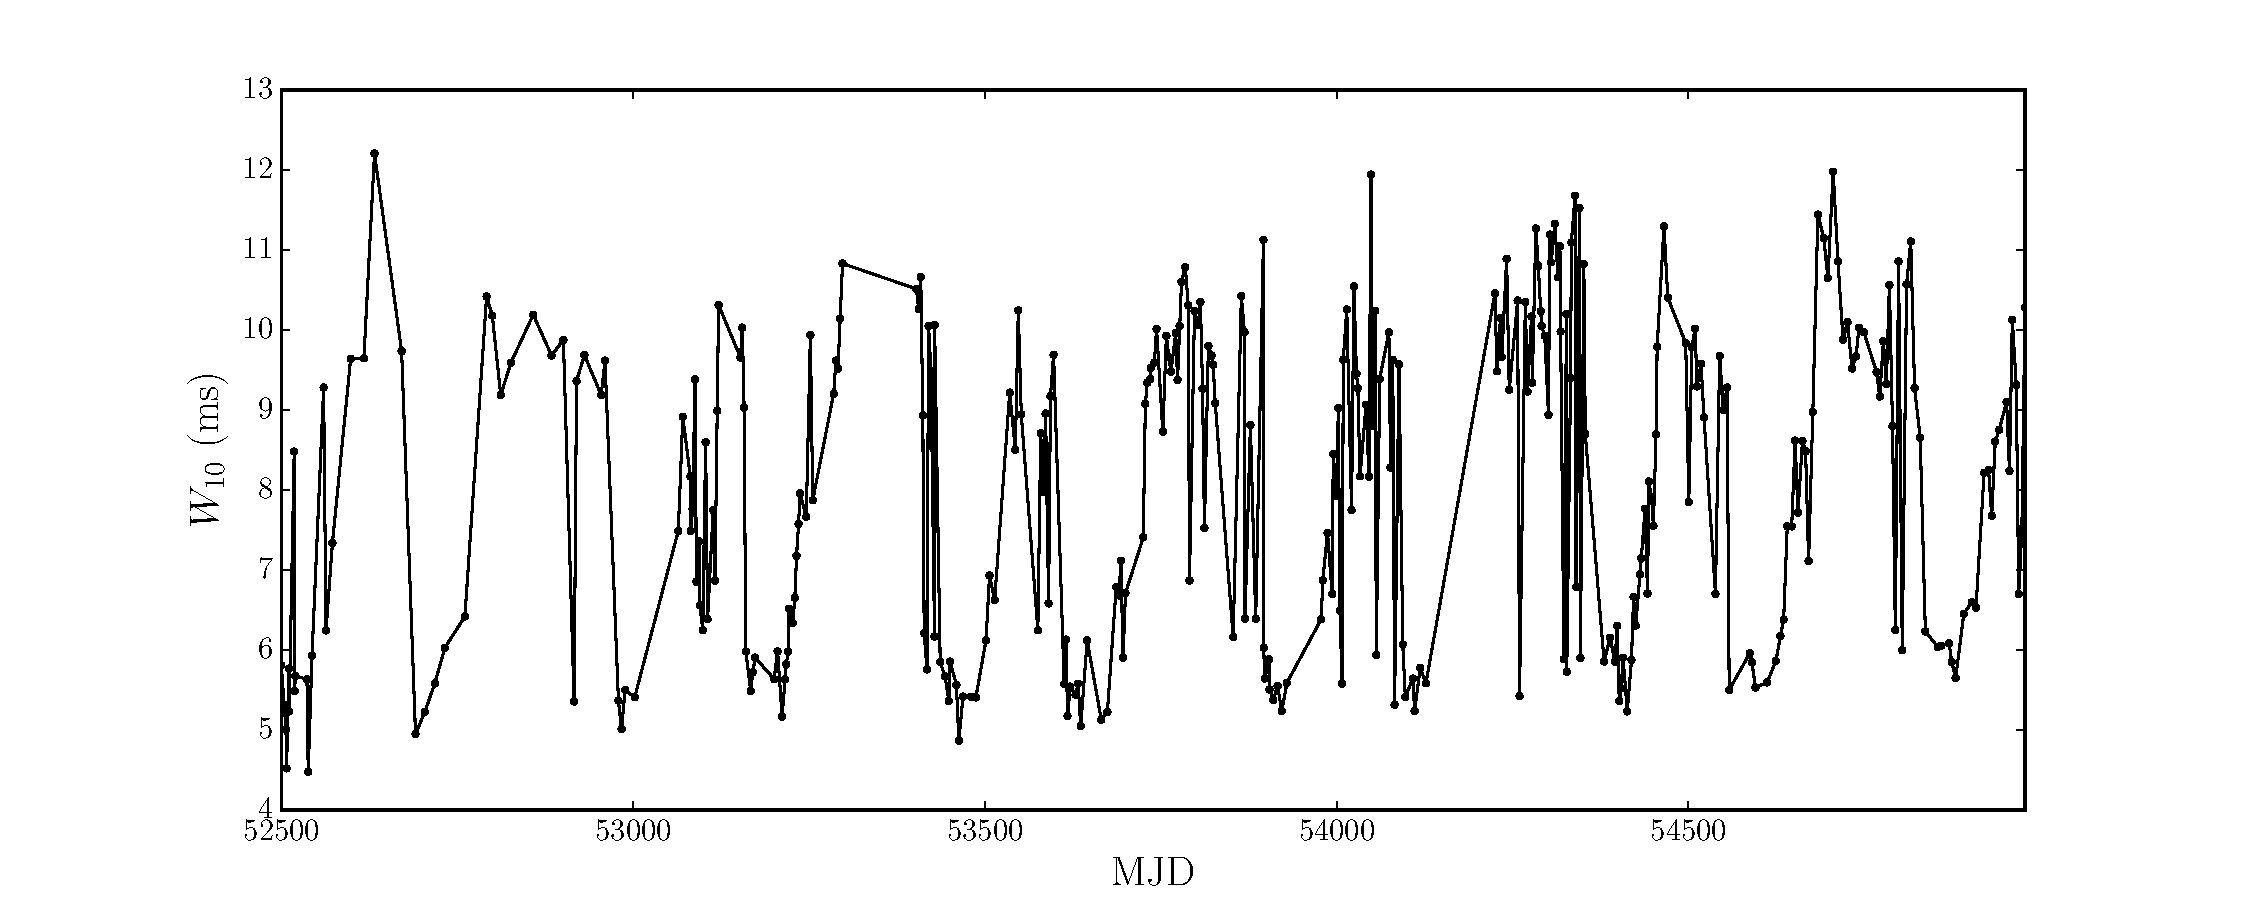
\includegraphics[width=.9\textwidth]{ExtractedData_B1828_W10_01.pdf}
    \caption{Raw data extracted from \citet{Lyne2010} on the $W_{10}$ value of
             B1828-11 which is a measure of the pulse width.}
    \label{fig: B1828 data}
\end{figure}

The authors argue that this data is showing the beam width switching discreetly
between two values with a period $0.73$ yr$^{-1}$.  We intend to apply some
data analysis to better understand this statement since there is some doubts
about the consistency of the measured values.

\FloatBarrier
\section{Histogram}
Since the claim centers on the fact that the beam width switches it makes sense
to begin by binning the measured values in a histogram. In figure \ref{fig: B1828 hist}
we show such a histogram corresponding to the data in figure \ref{fig: B1828 data}
\begin{figure}[htb]
    \centering
    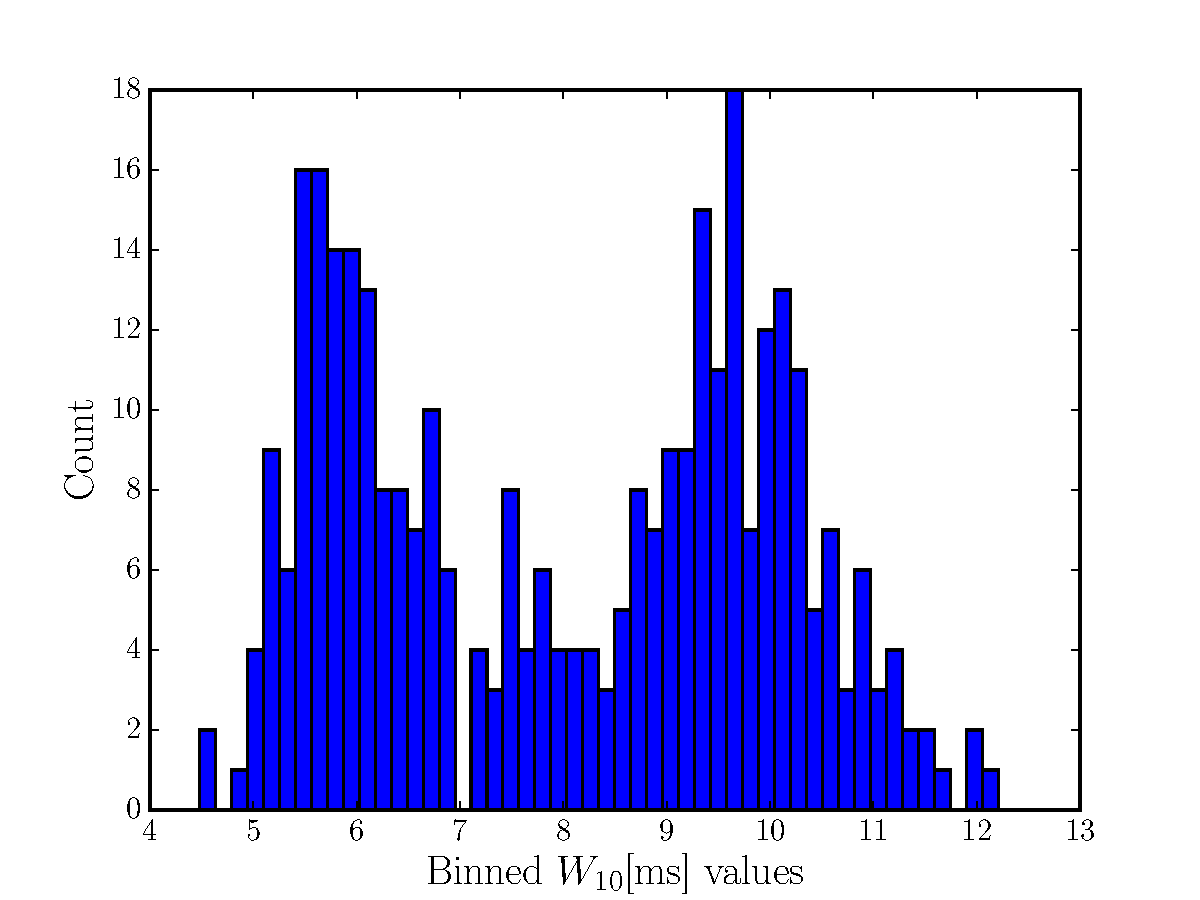
\includegraphics[width=.5\textwidth]{HistogramB1828_W10_01.pdf}
    \caption{A histogram of the data presented in figure \ref{fig: B1828 data}
             binned according the value of $W_{10}$. This clearly demonstrates
             a bimodal distribution.}
    \label{fig: B1828 hist}
\end{figure}

Evidently the histogram illustrates that the beam width follows a bi-modal
distribution. The Lyne hypthosis to explain this is:

\begin{itemize}

    \item[$\mathcal{H}_{\textrm{Lyne}}$:] The spin-down switches discreetly between two
        distinct values in a square-wave pattern. This is caused by changes in
        the magnetosphere which manifest as changes in the beam width.
        Therefore, the beam width must also follow a square wave pattern.

\end{itemize}

We would like to question the evidence for this hypothesis, by comparing with 
some alternatives. We now proceed to analyse competitor models with
the aim being to quantify which, if any, of the models best described the
observed data.

\FloatBarrier
\section{An alternative hypthesis: A trigonometric function}
\graphicspath{{/home/greg/Neutron_star_modelling/AnalysisLyneObservations/img/}}

The primary competitor model to the square wave which we consider will be a
simple trig. function. This is motivated by variations in the beam width due to
free precession (a model that itself has potential to describe the spin-down
variations). Free precession however procudes a complicates oscillatory
function that could be the sum of several harmonically related sinusoid.
Instead using a single sine-wave captures the idea that the beam width smoothly
varies rather than as a square-wave without introducing any additional
complexity. 

\subsection{Motivation using simple numerical example}

\subsubsection{Trig. function without noise}
We can begin by demonstrating why the hypothesis that figure \ref{fig: B1828
data} is uniquely described by a square-wave model is open to debate. To do
this we take a simply function such as
\begin{equation}
    y(x) = y_{0} + A \sin(\omega t) 
    \label{eqn: sin}
\end{equation}
Then writing a simple script which produces data for $x$ and $y$, we pick some 
number of random points from the data; this simulated the process of collecting
data. We can then `bin' the $y$ values in a histogram to look at their distribution.
This is done in figure \ref{fig: Sinx without noise} showing both the collected
points and their distribution.
\begin{figure}[htb]
    \centering
    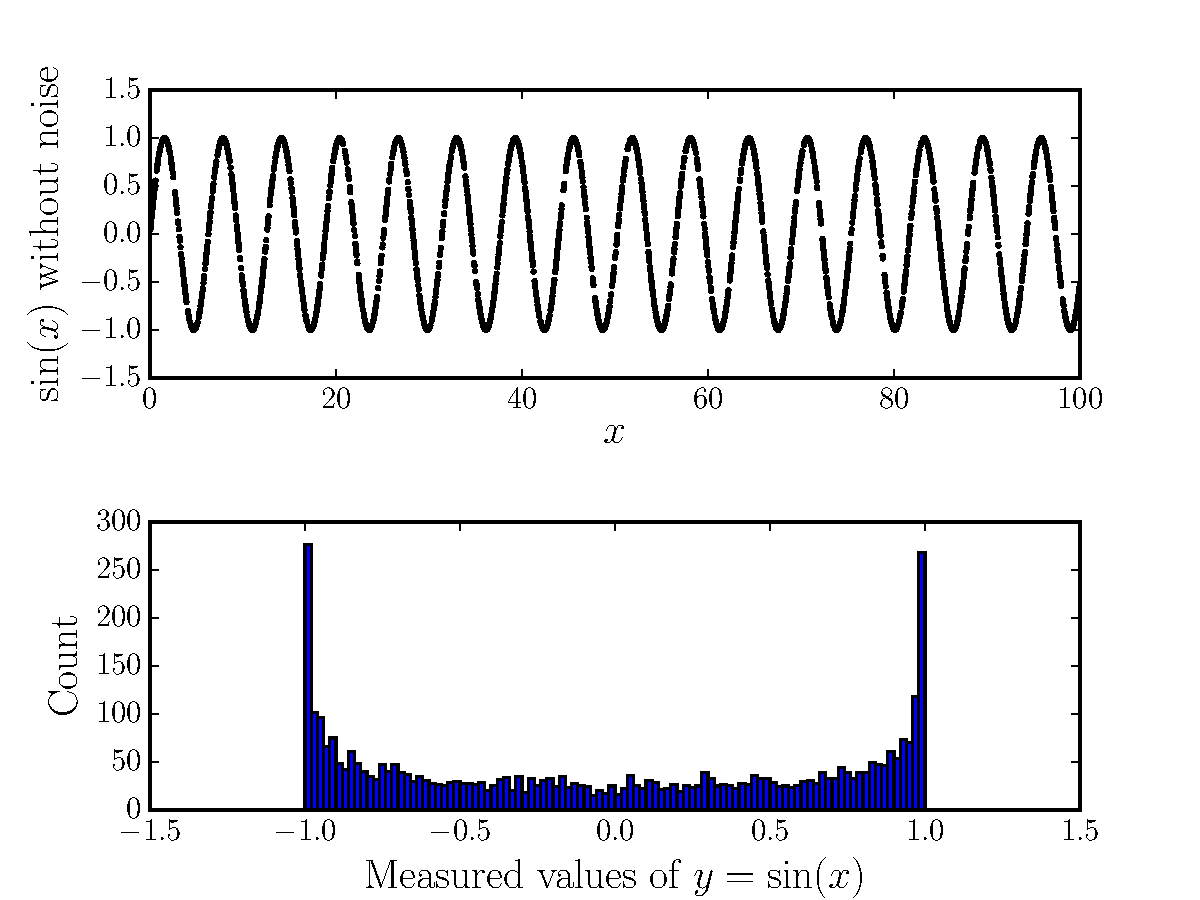
\includegraphics[width=0.6\textwidth]{Sinx_without_noise}
    \caption{In the top panel is the collected data for eqn. \eqref{eqn: sin} with
             $A=1$, $y_{0}=0$. In the lower panel is the binned data on the 
         collected values of $y$ in a histogram.}
    \label{fig: Sinx without noise}
\end{figure}
We note the particular shape of the histogram has two distinct peaks. This 
can be intuitively understood as the result of the system spending more time
near the extrema. 

This histogram result provides an insight at an underlying probability
distribution.  Namely, if we measure values from an oscillating system, what is
the probability of getting some particular value?  We analytically calculate
this underlying distribution in section \ref{sec: Analytic calculation sinx}.

\subsubsection{Trig. function with noise}

Cleary to fit with the observed data, we must also include a noise component
to avoid having a hard cutoff at $y = y_{0} \pm A$. This can be done by assuming
the noise is normally distributed such that
\begin{equation}
    y(x) = y_{0} + A \sin(\omega t) + \mathcal{N}(0, \sigma^{2})
    \label{eqn: sin + noise}
\end{equation}

We can again simulate this numerically and the result for a particular
realisation is given in figure \ref{fig: Sinx without noise}.
\begin{figure}[htb]
    \centering
    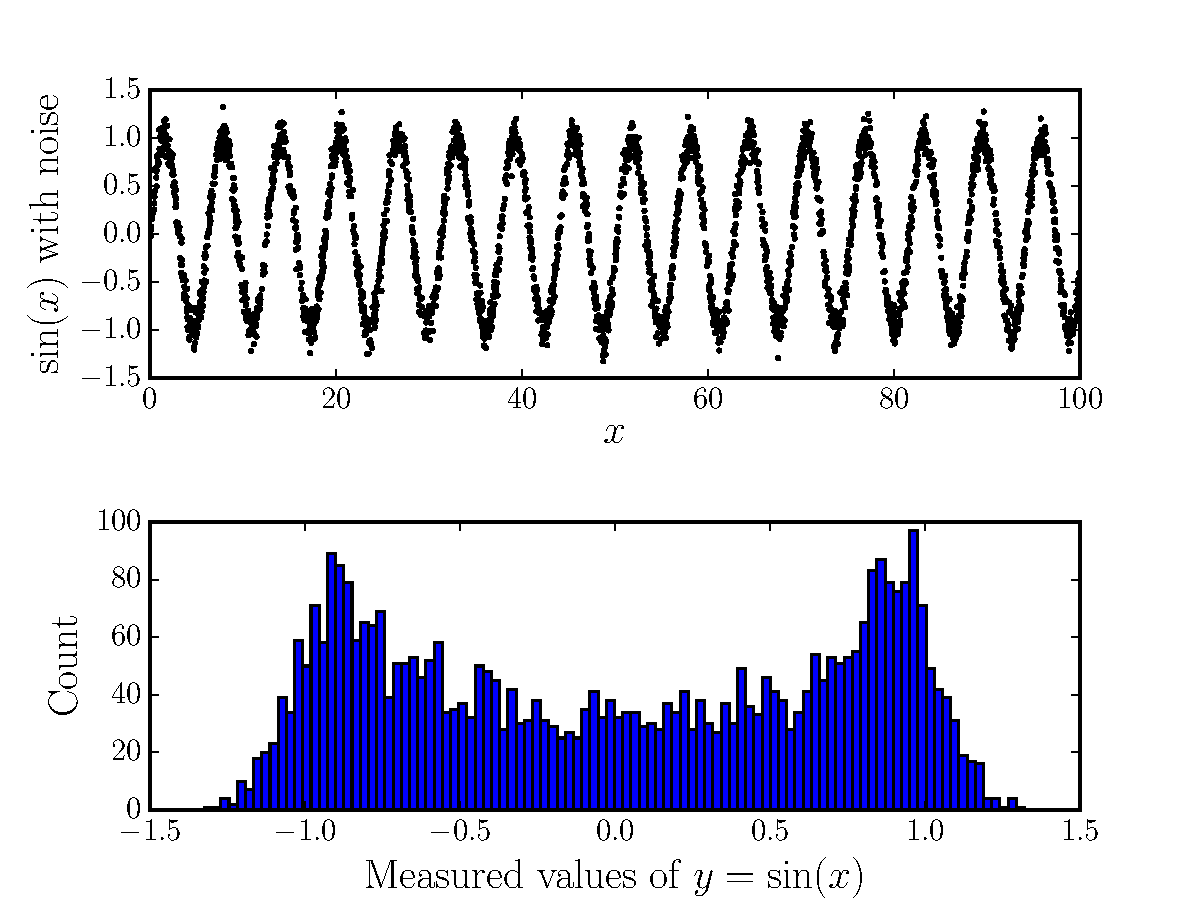
\includegraphics[width=0.6\textwidth]{Sinx_with_noise}
    \caption{In the top panel is the collected data for eqn. \eqref{eqn: sin + noise} with
             $A=1$, $y_{0}=0$ and $\sigma =0.1$. In the lower panel is the binned data on the 
         collected values of $y$ in a histogram.}
    \label{fig: Sinx with noise}
\end{figure}

The addition of noise notably broadens the histogram but can, if the noise is
sufficiently weak, retain the bimodal structure. 

\FloatBarrier
\subsection{Analytic calculation}
\label{sec: Analytic calculation sinx}
\subsubsection{Trig. function without noise}

As we have demonstrated, the histogram of values from randomly selecting points
on a sine wave is bi-modal. This suggests their is an underlying probability
distribution which we will now calculate.  That is, we can think of making a
measurement $y_{i}$ on the system, then the distribution from which this is
drawn is the underlying probability distribuition $f(y)$ which we wish to
calculate.  This can be calculated from the inverse-CDF method, however a
simpler and more intuitive approach follows.

Let us assume that we choose a point $x_{i}$ at which to measure the system, and
that the $x_{i}$ are uniformly distributed on $[0, X]$ where $X=\frac{2\pi}{\omega}$
is the period of the sine wave. Note that while we are considering picking points
over only a single period, this is the same as pick points over an arbitary 
number of periods since the sine-wave is a repetitive oscillation.

Since the $x_i$ are uniformly distributed, the probability density function for
$y$ must satisfy
\begin{equation}
    f(y)dy = \frac{dx}{X}.
\end{equation}
Inserting the definition for the period and rearranging
\begin{equation}
    f(y) = \frac{dt}{dy} \frac{\omega}{2\pi}.
\end{equation}
Inverting the relation between $y$ and $t$ and differentiating we end up with a 
normalised probability distribution
\begin{equation}
    f(y) = \frac{1}{2\pi A} \left(1 - \left(\frac{y - y_{0}}{A}\right)^{2}\right)^{-1/2}
    \label{eqn: P(y)}
\end{equation}
We plot the distribution in figure \ref{fig: SinDistribution} and can be qualitatively
compared with the histogram in \ref{fig: Sinx without noise} to verify that this
is the underlying probability distribution.
\begin{figure}[htb]
    \centering
    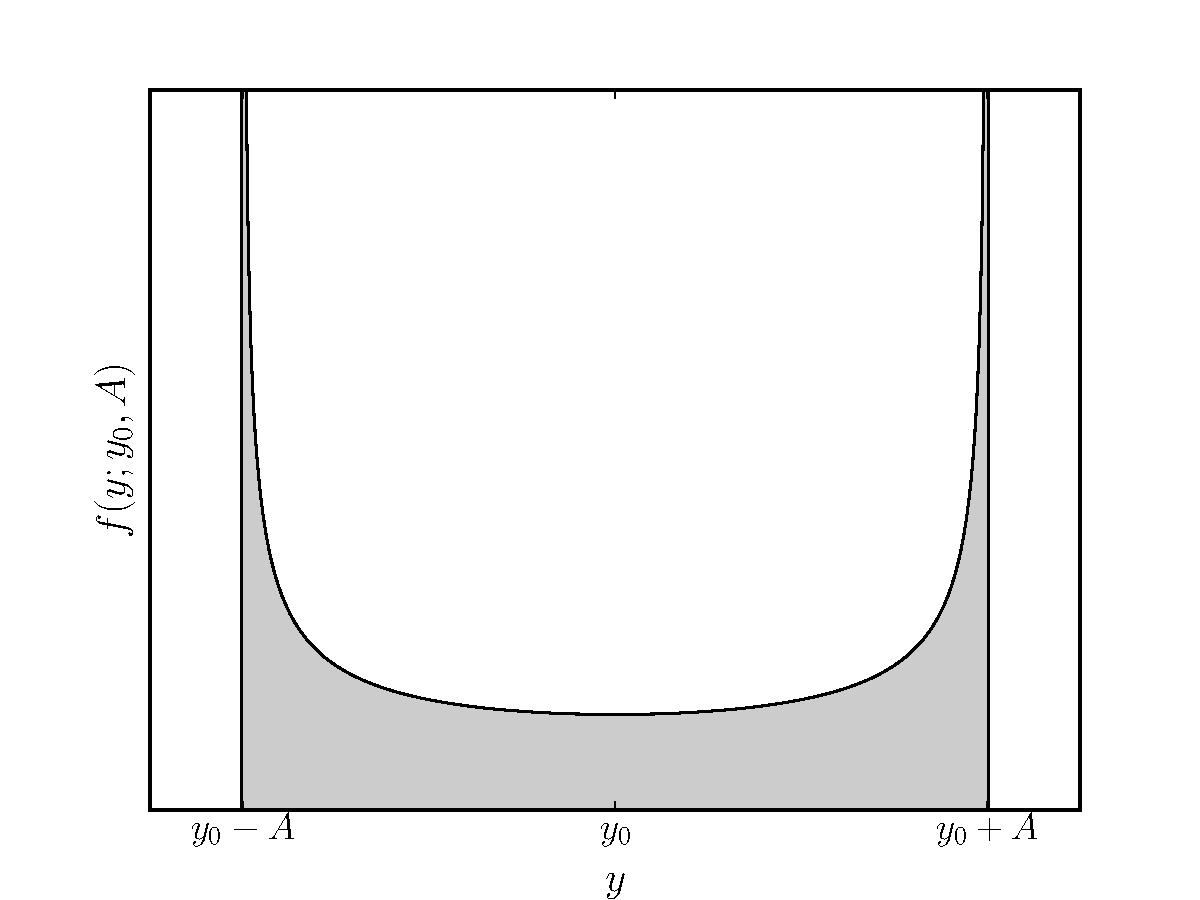
\includegraphics[width=0.6\textwidth]{SinDistribution.pdf}
    \caption{Plot of the probability density function in eqn. \eqref{eqn: P(y)}}
    \label{fig: SinDistribution}
\end{figure}

\subsubsection{Trig. function with noise}
Adding noise to each measurement means that our measured value $y_{i}^{M}$ is
given by 
\begin{equation}
    y_{i}^{M} = y_{i} + \epsilon_{i}
\end{equation}
where $y_{i}$ is the deterministic value with probability distribution given by
\eqref{eqn: P(y)} and $\epsilon_{i}$ is a random variable representing the 
error. This could be either an intrinsic error which depends in a complex
way on the properties of the $y_{i}$ or a measurement
error. In the latter case the distribution will be independant; this simplifies
the problem and so we consider only this case for now. Let the measurement error
be normally distributed such that
\begin{equation}
    \epsilon_{i} \sim N(0, \sigma^{2})
\end{equation}
then the probability density function is given by 
\begin{equation}
    g(\epsilon_{i}) = \frac{1}{\sigma\sqrt{2\pi}} \exp\{-\epsilon^{2}/2\sigma^{2}\}
\end{equation}

If the random variables $y_{i}$ and $\epsilon_i$ are independant, then the
probability distribution of the measured value (their sum) is
given by the convolution of their probability density functions:
\begin{align}
    P(y^{M}) = (f * g)(y) & = \int_{-\infty}^{\infty} f(\tilde{y}) g(y - \tilde{y}) d\tilde{y} \\
                          & = \frac{1}{2\pi A\sigma\sqrt{2\pi}} \int_{-\infty}^{\infty}
\frac{\exp\left\{-(y - \tilde{y})^{2}/2\sigma^{2}\right\}}
{\sqrt{(1 - \left((\tilde{y} - y_{0}) / A \right)^{2}}}
d\tilde{y}
\end{align}
This integration is not easy to analytically integrate. Nevertheless, we can 
calculate any particular realisation by numerical integration. In figure
\ref{fig: SinDistribution with noise} we plot the numerical integration for 
some particular values of $A$, $y_{0}$ and $\sigma$.
\begin{figure}[htb]
    \centering
    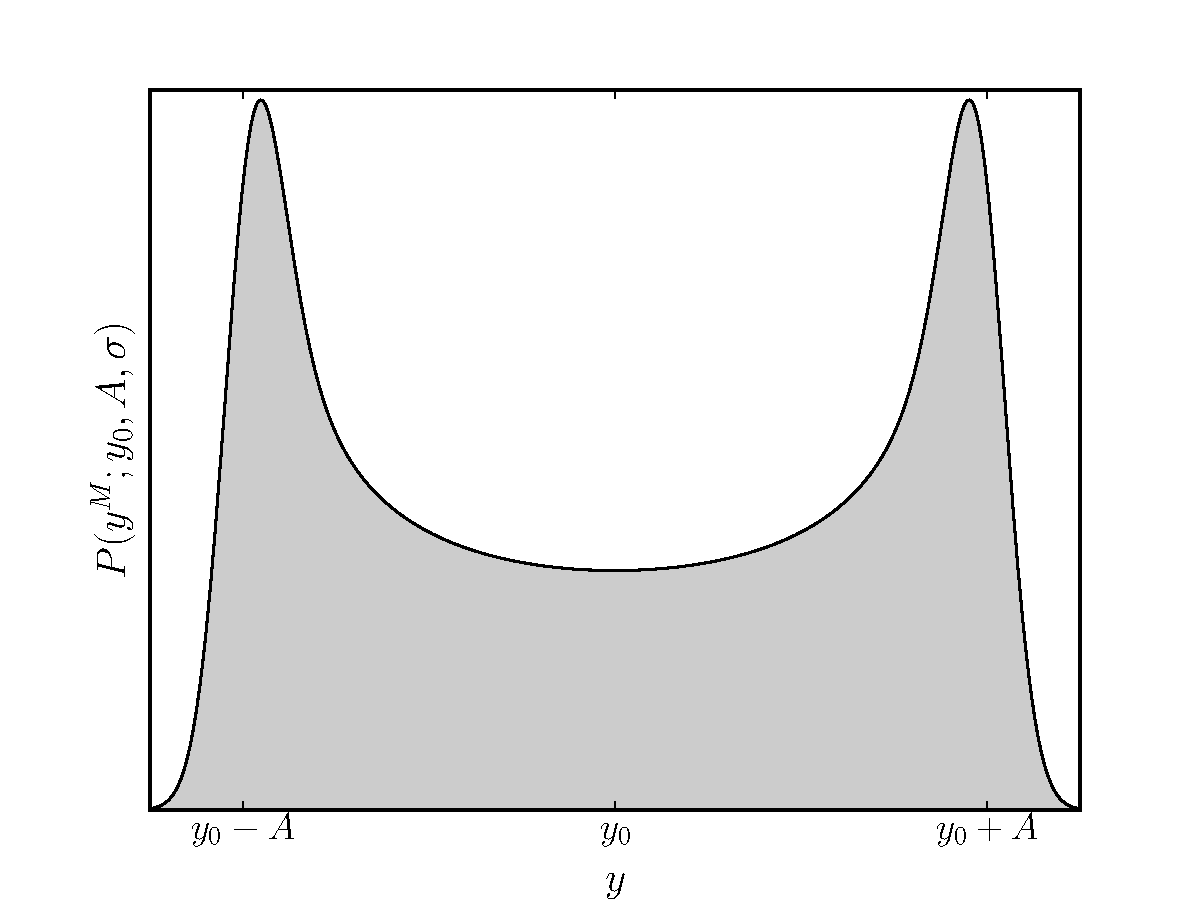
\includegraphics[width=0.6\textwidth]{SinDistribution_withnoise}
    \caption{A numerical calculation of the probability distribution resulting
             from the convolution of the noise process and the probability for
             picking values from a trig. function.}
    \label{fig: SinDistribution with noise}
\end{figure}


\biblio
\end{document}

